\subsection{View}

\class {Language}
public class Language

\begin{minipage}{0.3\textwidth}
    \begin{figure}[H]
        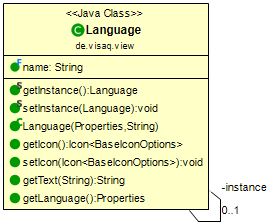
\includegraphics[scale = 0.5]{media/frontend/view/de.view/Language_Class.png}
    \end{figure}
\end{minipage} \hfill
\begin{minipage}{0.6\textwidth}
    Language wird benutzt um die Sprache nach den präferenzen des Benutzers zu setzen. Die Klasse ist nach dem Singelton Entwurfsschema designt.
\end{minipage}

Attribute:
\begin{itemize}
    \item \emph{public final String name} Name der Sprache
\end{itemize}
Methoden:
\begin{itemize}
    \item \emph{public static synchronized Language getInstance()} Gibt die aktuelle Sprach-Instanz wieder.
    \item \emph{public static synchronized void setInstance(Language language)} Setzt die aktuelle Sprach-Instanz
    \item \emph{public Language(Properties language, String name)} Konstruktor, welcher die Sprache mit dem gegebenen Namen erstellt und die globale Instanz dementsprechend aktualisiert.
    \item \emph{public Icon<BaseIconOptions> getIcon()} Gibt das Icon wieder, welches in der Navigationsbar angezeigt wird.
    \item \emph{public void setIcon(Icon<BaseIconOptions> icon)} Setzt das Icon
    \item \emph{public String getText(String key)} Gibt die lokalisierte Version des Property key zurück
    \item \emph{public Properties getLanguage()} Wird benutzt um die Sprach Properties zu erreichen
\end{itemize}

\rule{\textwidth}{0.4pt}
\class{InformationView}
public class InformationView extends View
\\\\
\begin{minipage}{0.4\textwidth}
    \begin{figure}[H]
        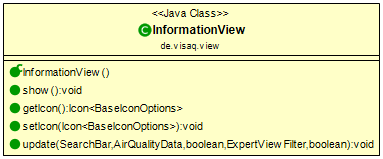
\includegraphics[scale = 0.5]{media/frontend/view/de.view/InformationView_Class.png}
    \end{figure}
\end{minipage} \hfill
\begin{minipage}{0.5\textwidth}
    InformationView erstellt die View mit welcher die Benutzer ein hilfestellendes Overlay aktivieren können, um so leichter
    die Webanwendung zu navigieren.
\end{minipage}

Methoden:
\begin{itemize}
    \item \emph{public void show()} Zeigt das Hilfeoverlay an
    \item \emph{public Icon<BaseIconOptions> getIcon()} Gibt das Icon für die InformationView wieder
    \item \emph{public void setIcon(Icon<BaseIconOptions> icon)} Setzt das Icon für die InformationView, bei welchem es sich um ein Icon aus der Bibliothek \gls{Leaflet} handelt.
    \item \emph{public void update(SearchBar searchbar, AirQualityData currentAirQualityData, boolean expertView, ExpertViewFilter expertViewFilter, boolean historicalView)} Aktualisiert Instanzen der View. Die Methode wird von Klassen, die ObservedNavbarSubject implementieren aufgerufen, falls der Benutzer etwas an den Einstellungen ändert. Aktualisiert werden die Suchleiste, die aktuelle AirQualityData, der ExpertView, der ExpertViewFilter und die HistoricalView.
\end{itemize}

\rule{\textwidth}{0.4pt}
\class{MapView}
public class MapView extends View

\begin{minipage}{0.4\textwidth}
    \begin{figure}[H]
        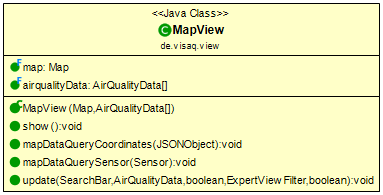
\includegraphics[scale = 0.5]{media/frontend/view/de.view/MapView_Class.png}
    \end{figure}
\end{minipage} \hfill
\begin{minipage}{0.5\textwidth}
    MapView erstellt die View für die Karte indem das MapOverlay angezeigt wird. Die Klasse erbt von View.
\end{minipage}

Attribute:
\begin{itemize}
    \item \emph{public final Map map} Die auf der Webanwendung angezeigte Karte
    \item \emph{public final AirQualityData[] airQualityData} Alle auf der Karte darstellbaren Luftqualitätsdaten.
\end{itemize}
Methoden:
\begin{itemize}
    \item \emph{public MapView(Map map,AirQualityData[] airQualityData)} Ein Konstruktor, welcher die Karte mit der aktuellen AirQualityData setzt.
    \item \emph{public void show()} Zeigt die Karte und Legende in der Webanwendung in dem Browser des Benutzers
    \item \emph{public void mapDataQueryCoordinates(JSONObject coordinates)} Wird aktiviert, wenn der Benutzer einen Punkt auf der Karte wählt. Zeigt die SensorOveriew mit den dazugehörigen Informationen an.
    \item \emph{public void mapDataQuerySensor(Sensor sensor)} Wird aktiviert, wenn der Benutzer einen Sensor auf der Karte wählt. Zeigt die SensorOveriew mit den dazugehörigen Informationen an.
    \item \emph{public void update(SearchBar searchBar, AirQualityData currentAirQualityData,
              boolean expertView, ExpertViewFilter expertViewFilter, boolean historicalView)} Aktualisiert Instanzen der View. Die Methode wird von Klassen, die ObservedNavbarSubject implementieren aufgerufen, falls der Benutzer etwas an den Einstellungen ändert. Aktualisiert werden die Suchleiste, die aktuelle AirQualityData, der ExpertView, der ExpertViewFilter und die HistoricalView.
\end{itemize}

\rule{\textwidth}{0.4pt}
\class{NavbarObserver}
public interface NavbarObserver

\begin{minipage}{0.4\textwidth}
    \begin{figure}[H]
        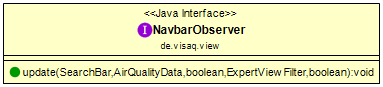
\includegraphics[scale = 0.5]{media/frontend/view/de.view/NavbarObserver_Class.png}
    \end{figure}
\end{minipage} \hfill
\begin{minipage}{0.5\textwidth}
    Ein Observer für die Navigationsbar welcher die Instanzen in dieser aktualisiert. Es handelt sich hierbei um ein Element aus dem Beobachter Entwurfsmuster. Der Observer ist ein Interface.
\end{minipage}

Methoden:
\begin{itemize} 
    \item \emph{public void update(SearchBar searchbar, AirQualityData currentAirQualityData,
    boolean expertView, ExpertViewFilter expertViewFilter, boolean historicalView)} Updaten der Navigationbar und ihrer Instanzen falls der Benutzer etwas an den Einstellungen ändert. Aktualisiert werden die Suchleiste, die aktuelle AirQualityData, der ExpertView, der ExpertViewFilter und die HistoricalView
\end{itemize}

\rule{\textwidth}{0.4pt}
\class{View}
public abstract class View implements NavbarObserver

\begin{minipage}{0.3\textwidth}
    \begin{figure}[H]
        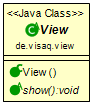
\includegraphics[scale = 0.7]{media/frontend/view/de.view/View_Class.png}
    \end{figure}
\end{minipage} \hfill
\begin{minipage}{0.7\textwidth}
    Eine abstrakte Klasse, welche regelt wie die Webanwendung für den Benutzer dargestellt wird. Das beinhaltet unter anderem die unterschiedlichen Sprachen und die ColorTheme. Die Klasse implementiert den NavbarObserver.
\end{minipage}

Methoden:
\begin{itemize}
    \item \emph{public void show()} Zeigt die unterschiedlichen Sektionen der Webanwendung
\end{itemize}

\rule{\textwidth}{0.4pt}
\class{VisAQ}
public class VisAQ

\begin{minipage}{0.3\textwidth}
    \begin{figure}[H]
        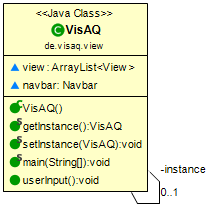
\includegraphics[scale = 0.6]{media/frontend/view/de.view/VisAQ_Class.png}
    \end{figure}
\end{minipage} \hfill
\begin{minipage}{0.6\textwidth}
    Die Main Klasse der Anwendung. Hier ist der Einstieg in die Anwendung, welcher die Eingaben des Benutzers weitergibt und die View öffnet. Dies erfolgt über das \gls{Angular-4-Candy} von \gls{Jsweet}. Die Klasse ist nach dem Singelton Entwurfsschema designt.
\end{minipage}

Methoden:
\begin{itemize}
    \item \emph{public static synchronized VisAQ getInstance()} Gibt eine VisAQ Instanz zurück
    \item \emph{public static synchronized void setInstance(VisAQ visAQ)} Setzt die VisAQ Instanz.
    \item \emph{public static void main(String[] args)} Die main-Methode der Anwendung. Hier startet die Webanwendung.
    \item \emph{public void userInput()} Informiert die Navbar, dass eine Nutzereingabe stattgefunden hat. Die Methode löst aus, dass die Navbar alle ihre Beobachter, die Views, aktualisiert.
\end{itemize}
